\def \imgpath {"./figures/alice"}


\begin{figure}%[!h]
\centering%
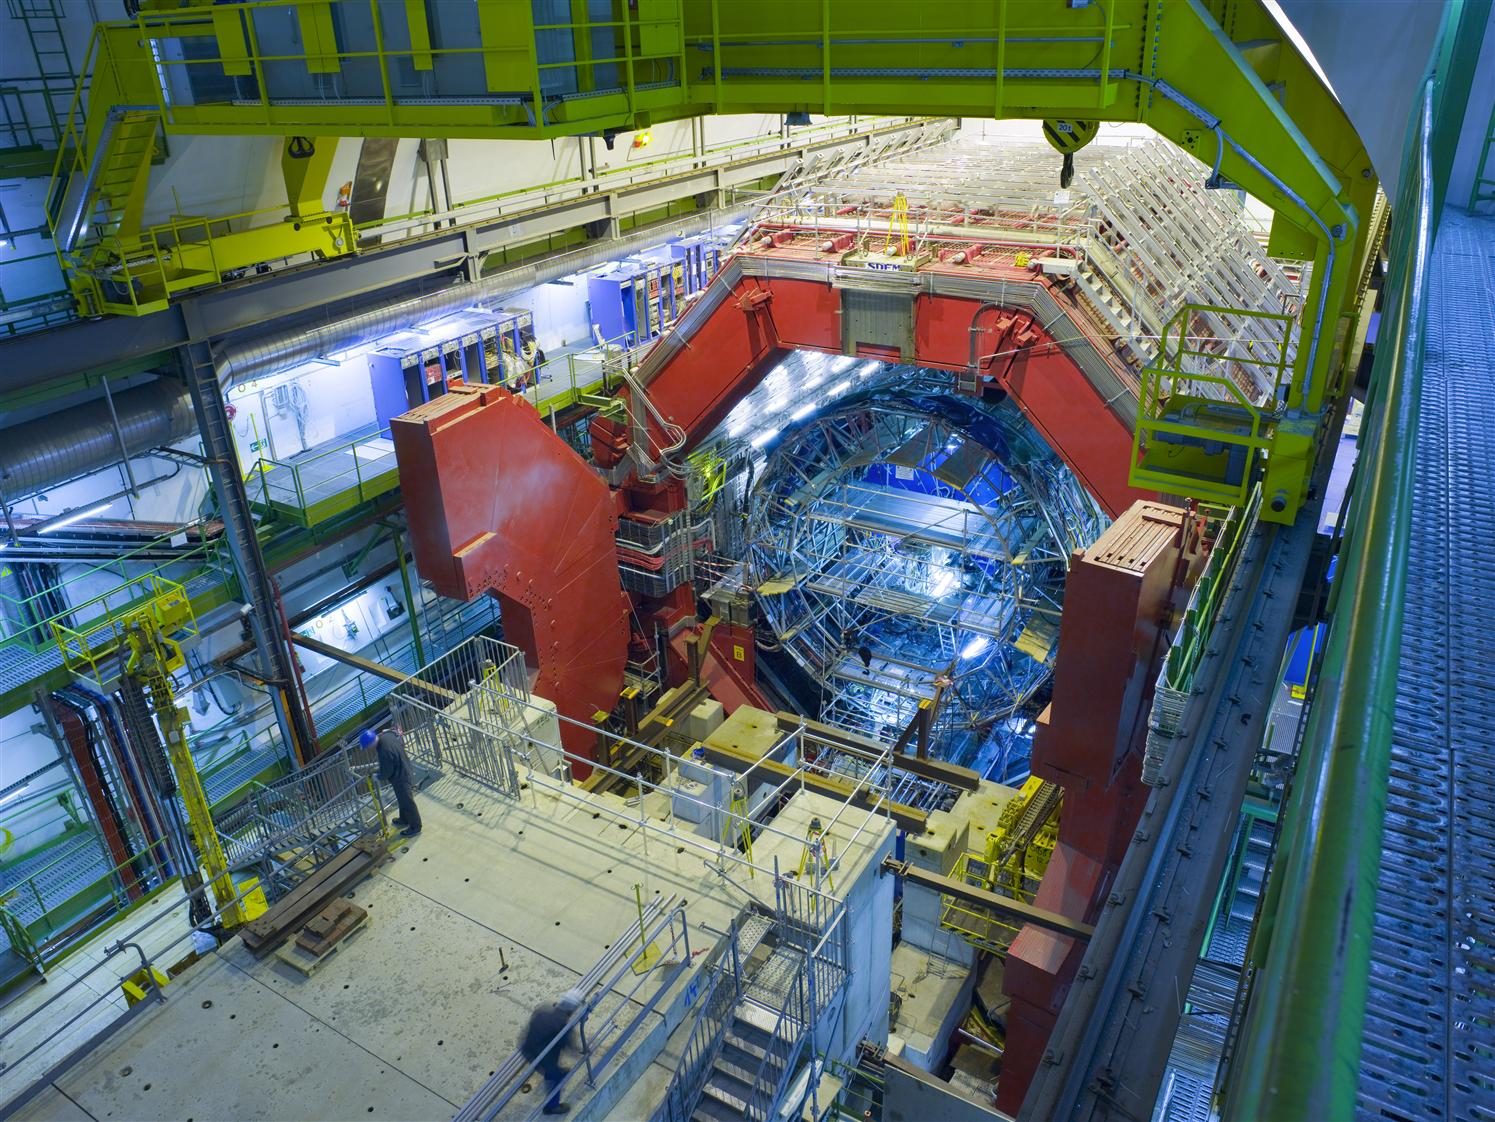
\includegraphics[width=.7\textwidth]{\imgpath/alicephoto.jpg}
\caption{TBA.}
\label{fig:experiment:cern}
\end{figure}

The ALICE (A Large Ion Collider Experiment) is one of four major detectors located at the Large Hadron Collider (LHC) at CERN. The ALICE detector is designed to study the properties of the quark-gluon plasma (QGP), a state of matter that existed a few microseconds after the Big Bang.

The ALICE detector consists of several sub-detectors that work together to capture and analyze the particles produced by the collisions at the LHC. The central component of the ALICE detector is the Time Projection Chamber (TPC), a large cylinder filled with a gas mixture that is used to detect the charged particles produced by the collisions. The TPC measures the position, momentum, and energy of the particles, allowing scientists to reconstruct their trajectories and identify the different particle species.

In addition to the TPC, the ALICE detector also includes several other sub-detectors, such as the Inner Tracking System (ITS), the Transition Radiation Detector (TRD), and the Time-Of-Flight (TOF) detector. The ITS is a high-precision tracking detector that is used to measure the trajectories of charged particles produced in the collisions. The TRD is used to identify electrons and measure their energy. The TOF detector measures the time-of-flight of particles and is used to determine their momentum.

\begin{figure}%[!h]
\centering%
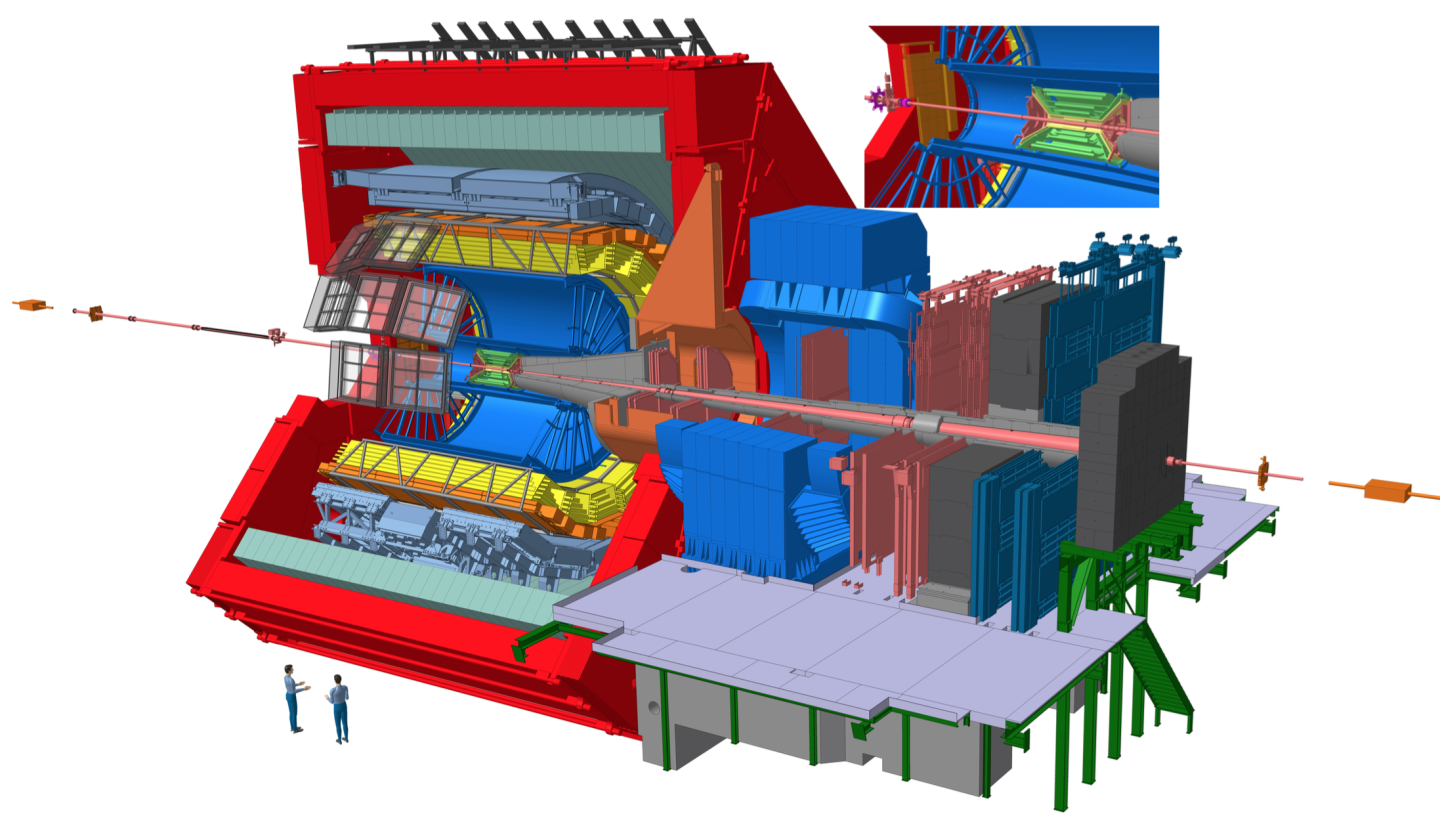
\includegraphics[width=.7\textwidth]{\imgpath/alicescheme2.png}
\caption{TBA.}
\label{fig:experiment:cern}
\end{figure}


\begin{figure}%[!h]
\centering%
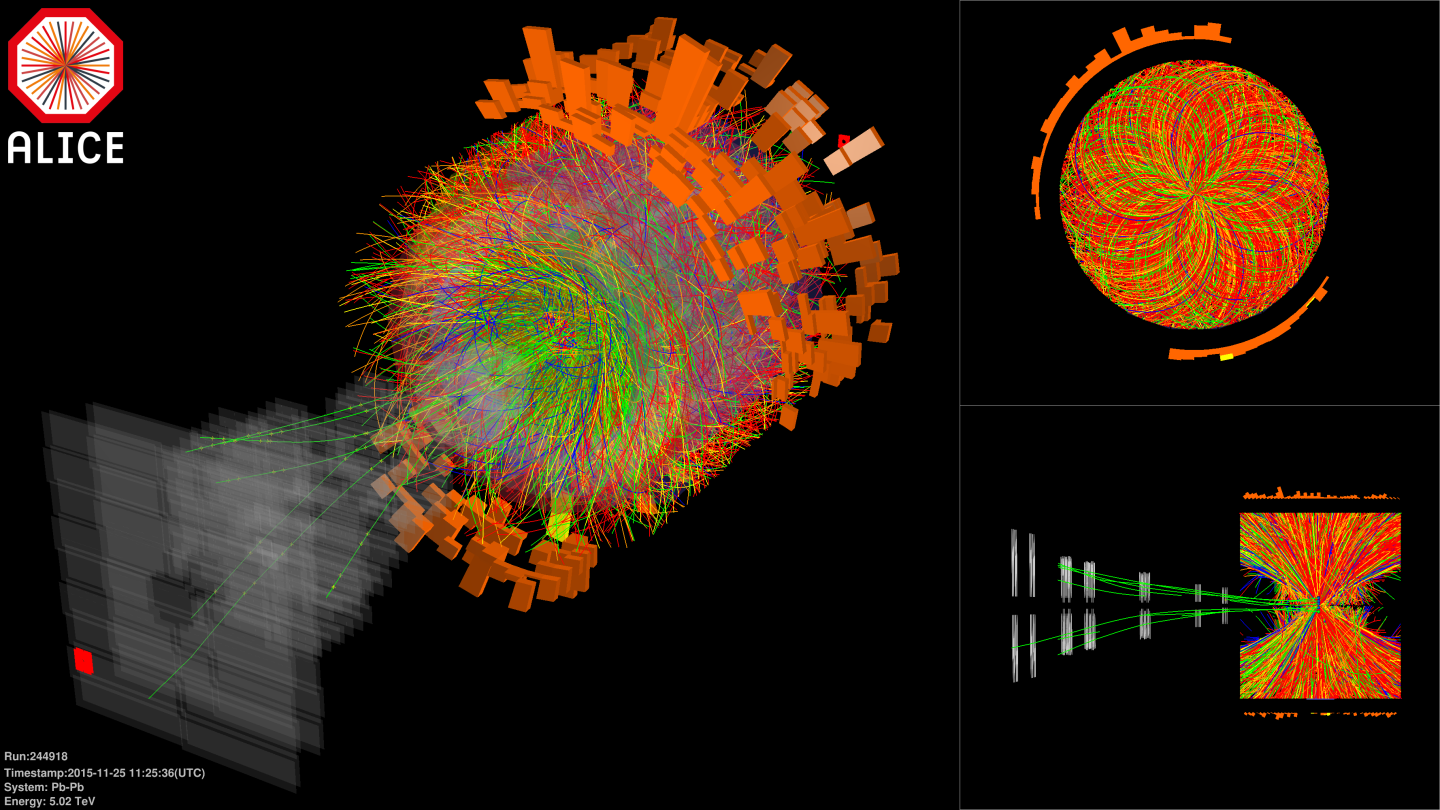
\includegraphics[width=.7\textwidth]{\imgpath/aliceevent.png}
\caption{TBA.}
\label{fig:experiment:cern}
\end{figure}

\section{Time Projection Chamber}

The TPC works by filling the cylinder with a gas, typically a mixture of helium and carbon dioxide, and applying an electric field to create a uniform drift velocity for the charged particles. As the particles move through the gas, they ionize the atoms, creating free electrons and ions. The electrons are then attracted to a central anode, where they are detected and used to reconstruct the particle tracks.

The TPC has a number of advantages over other types of detectors. For one, it is able to provide precise measurements of the position and momentum of the charged particles, which allows scientists to study the behavior of quark-gluon plasma and other forms of matter at extremely high temperatures and densities. The TPC is also able to reconstruct the tracks of thousands of particles produced in a single collision, which provides a comprehensive view of the event.

The TPC in the ALICE experiment is particularly advanced, with over 500,000 readout channels and a sensitive volume of over 90 cubic meters. It is able to operate at high collision rates, with a maximum readout rate of 50 kHz. The TPC also has a number of innovative features, such as a gating system that allows the detector to operate in the presence of large magnetic fields, and a continuous calibration system that ensures high data quality.


\begin{figure}%[!h]
\centering%
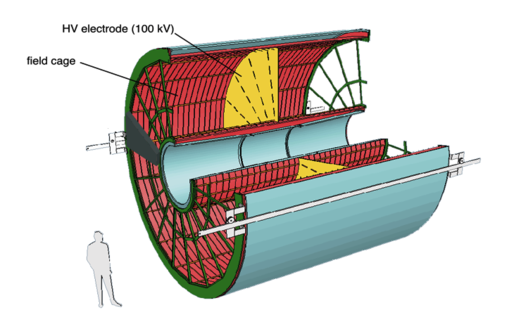
\includegraphics[width=.7\textwidth]{\imgpath/alicetpc.png}
\caption{TBA.}
\label{fig:experiment:cern}
\end{figure}


\section{Inner Tracking Systems}

The ITS is another tracking detector in the ALICE experiment, located closer to the collision point than the TPC. It is designed to provide precise measurements of the position of charged particles as they are produced in the collisions. The ITS consists of six layers of silicon detectors, which provide high-resolution measurements of the position and momentum of the particles. The ITS is particularly useful for studying the very early stages of the collision, where the particles are produced in a very small volume and with high energies.


\begin{figure}%[!h]
\centering%
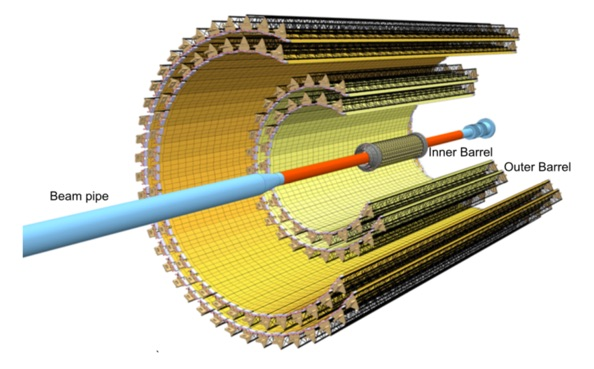
\includegraphics[width=.7\textwidth]{\imgpath/aliceits.jpg}
\caption{TBA.}
\label{fig:experiment:cern}
\end{figure}
